\documentclass[12pt, titlepage]{article}

\usepackage{fullpage}
\usepackage[round]{natbib}
\usepackage{multirow}
\usepackage{booktabs}
\usepackage{tabularx}
\usepackage{graphicx}
\usepackage{float}
\usepackage{hyperref}
\hypersetup{
    colorlinks,
    citecolor=blue,
    filecolor=black,
    linkcolor=red,
    urlcolor=blue
}

%% Comments

\usepackage{color}

\newif\ifcomments\commentstrue

\ifcomments
\newcommand{\authornote}[3]{\textcolor{#1}{[#3 ---#2]}}
\newcommand{\todo}[1]{\textcolor{red}{[TODO: #1]}}
\else
\newcommand{\authornote}[3]{}
\newcommand{\todo}[1]{}
\fi

\newcommand{\wss}[1]{\authornote{blue}{SS}{#1}} 
\newcommand{\plt}[1]{\authornote{magenta}{TPLT}{#1}} %For explanation of the template
\newcommand{\an}[1]{\authornote{cyan}{Author}{#1}}

%% Common Parts

\newcommand{\progname}{ProgName} % PUT YOUR PROGRAM NAME HERE %Every program
                                % should have a name


\newcounter{acnum}
\newcommand{\actheacnum}{AC\theacnum}
\newcommand{\acref}[1]{AC\ref{#1}}

\newcounter{ucnum}
\newcommand{\uctheucnum}{UC\theucnum}
\newcommand{\uref}[1]{UC\ref{#1}}

\newcounter{mnum}
\newcommand{\mthemnum}{M\themnum}
\newcommand{\mref}[1]{M\ref{#1}}

\begin{document}

\title{Module Guide for EOMEE} 
\author{Gabriela S\'anchez D\'iaz}
\date{\today}

\maketitle

\pagenumbering{roman}

\section{Revision History}

\begin{tabularx}{\textwidth}{p{3cm}p{2cm}X}
\toprule {\bf Date} & {\bf Version} & {\bf Notes}\\
\midrule
20-11-2020 & 1.0 & MG first draft\\
%Date 2 & 1.1 & Notes\\
\bottomrule
\end{tabularx}

\newpage

\section{Reference Material}

This section records information for easy reference.

\subsection{Abbreviations and Acronyms}

\renewcommand{\arraystretch}{1.2}
\begin{tabular}{l l} 
  \toprule		
  \textbf{symbol} & \textbf{description}\\
  \midrule 
  AC & Anticipated Change\\
  DAG & Directed Acyclic Graph \\
  M & Module \\
  MG & Module Guide \\
  OS & Operating System \\
  R & Requirement\\
  SC & Scientific Computing \\
  SRS & Software Requirements Specification\\
  \progname & Explanation of program name\\
  UC & Unlikely Change \\
  EOM & Equation of motion\\
  RDM & Reduced Density Matrix\\
  TDM & Transition Density Matrix\\
  \bottomrule
\end{tabular}\\

See also the corresponding section in the SRS Documentation at 
\href{https://github.com/gabrielasd/eomee/tree/cas741/docs/SRS/}{SRS}.\\
\newpage

\tableofcontents

\listoftables

\listoffigures

\newpage

\pagenumbering{arabic}

\section{Introduction}

Decomposing a system into modules is a commonly accepted approach to developing
software.  A module is a work assignment for a programmer or programming
team~\citep{ParnasEtAl1984}.  We advocate a decomposition
based on the principle of information hiding~\citep{Parnas1972a}.  This
principle supports design for change, because the ``secrets'' that each module
hides represent likely future changes.  Design for change is valuable in SC,
where modifications are frequent, especially during initial development as the
solution space is explored.  

Our design follows the rules layed out by \citet{ParnasEtAl1984}, as follows:
\begin{itemize}
\item System details that are likely to change independently should be the
  secrets of separate modules.
\item Each data structure is implemented in only one module.
\item Any other program that requires information stored in a module's data
  structures must obtain it by calling access programs belonging to that module.
\end{itemize}

After completing the first stage of the design, the Software Requirements
Specification (SRS), the Module Guide (MG) is developed~\citep{ParnasEtAl1984}. The MG
specifies the modular structure of the system and is intended to allow both
designers and maintainers to easily identify the parts of the software.  The
potential readers of this document are as follows:

\begin{itemize}
\item New project members: This document can be a guide for a new project member
  to easily understand the overall structure and quickly find the
  relevant modules they are searching for.
\item Maintainers: The hierarchical structure of the module guide improves the
  maintainers' understanding when they need to make changes to the system. It is
  important for a maintainer to update the relevant sections of the document
  after changes have been made.
\item Designers: Once the module guide has been written, it can be used to
  check for consistency, feasibility and flexibility. Designers can verify the
  system in various ways, such as consistency among modules, feasibility of the
  decomposition, and flexibility of the design.
\end{itemize}

The rest of the document is organized as follows. Section
\ref{SecChange} lists the anticipated and unlikely changes of the software
requirements. Section \ref{SecMH} summarizes the module decomposition that
was constructed according to the likely changes. Section \ref{SecConnection}
specifies the connections between the software requirements and the
modules. Section \ref{SecMD} gives a detailed description of the
modules. Section \ref{SecTM} includes two traceability matrices. One checks
the completeness of the design against the requirements provided in the SRS. The
other shows the relation between anticipated changes and the modules. Section
\ref{SecUse} describes the use relation between modules.

\section{Anticipated and Unlikely Changes} \label{SecChange}

This section lists possible changes to the system. According to the likeliness
of the change, the possible changes are classified into two
categories. Anticipated changes are listed in Section \ref{SecAchange}, and
unlikely changes are listed in Section \ref{SecUchange}.

\subsection{Anticipated Changes} \label{SecAchange}

Anticipated changes are the source of the information that is to be hidden
inside the modules. Ideally, changing one of the anticipated changes will only
require changing the one module that hides the associated decision. The approach
adapted here is called design for
change.

\begin{description}
\item[\refstepcounter{acnum} \actheacnum \label{acHardware}:] The specific
  hardware on which the software is running and the libraries 
  provided by the programming language.
\item[\refstepcounter{acnum} \actheacnum \label{acInput}:] The
initial input data (its format and number of parameters).
\item[\refstepcounter{acnum} \actheacnum \label{acDriver}:] How the different 
routines are called.
\item[\refstepcounter{acnum} \actheacnum \label{acIntegrals}:] The format of 
the electron integrals (given in molecular orbital basis or spin orbitals basis)
\item[\refstepcounter{acnum} \actheacnum \label{acRDMs}:] The input format of 
the density matrices.
\item[\refstepcounter{acnum} \actheacnum \label{acEOMs}:] The Equation of 
motion (EOM) methods (more equation definitions could be added).
\item[\refstepcounter{acnum} \actheacnum \label{acTDMs}:] How the transition 
density matrices (TDMs) are implemented.
\item[\refstepcounter{acnum} \actheacnum \label{acSolver}:] How the EOMs are 
solved.
\item[\refstepcounter{acnum} \actheacnum \label{acOutput}:] The output data 
format.
\end{description}

\subsection{Unlikely Changes} \label{SecUchange}

The module design should be as general as possible. However, a general system is
more complex. Sometimes this complexity is not necessary. Fixing some design
decisions at the system architecture stage can simplify the software design. If
these decision should later need to be changed, then many parts of the design
will potentially need to be modified. Hence, it is not intended that these
decisions will be changed.

\begin{description}
\item[\refstepcounter{ucnum} \uctheucnum \label{ucIO}:] Input/Output devices
  (Input: File and/or Keyboard, Output: File, Memory, and/or Screen).
\item[\refstepcounter{ucnum} \uctheucnum \label{ucRDMs}:] How the EOMs are 
defined in terms of the one- and two-electron integrals and RDMs.
\item[\refstepcounter{ucnum} \uctheucnum \label{ucGenEigval}:] The 
representation of the EOM as a generalized eigenvalue problem.
\end{description}

\section{Module Hierarchy} \label{SecMH}

This section provides an overview of the module design. Modules are summarized
in a hierarchy decomposed by secrets in Table \ref{TblMH}. The modules listed
below, which are leaves in the hierarchy tree, are the modules that will
actually be implemented.

\begin{description}
\item [\refstepcounter{mnum} \mthemnum \label{mHH}:] Hardware-Hiding Module
\item [\refstepcounter{mnum} \mthemnum \label{mDriver}:] Control Module
\item [\refstepcounter{mnum} \mthemnum \label{mInput}:] Input Module
\item [\refstepcounter{mnum} \mthemnum \label{mIntegrals}:] Integrals Module
\item [\refstepcounter{mnum} \mthemnum \label{mRDMs}:] Reduced density matrices 
(RDMs) Module 
\item [\refstepcounter{mnum} \mthemnum \label{mEOM}:] EOM Interface Module
\item [\refstepcounter{mnum} \mthemnum \label{mEOMIP}:] IP EOM Module
\item [\refstepcounter{mnum} \mthemnum \label{mEOMEA}:] EA EOM Module
\item [\refstepcounter{mnum} \mthemnum \label{mEOMExc}:] Excitation EOM Module
\item [\refstepcounter{mnum} \mthemnum \label{mEOMDIP}:] DIP EOM Module
\item [\refstepcounter{mnum} \mthemnum \label{mEOMDEA}:] DEA EOM Module
%\item [\refstepcounter{mnum} \mthemnum \label{mTDM}:] TDM module
\item [\refstepcounter{mnum} \mthemnum \label{mGEP}:] Generalized Eigenvalue 
Solver Module.
\item [\refstepcounter{mnum} \mthemnum \label{mOutput}:] Output Module
\end{description}
Note that module M\ref{mHH}, corresponding to the libraries provided by the 
operative system, is not going to be reimplemented. Also, the solver module 
M\ref{mGEP} is a partial implementation given that it uses a linear solver and 
singular value decomposition algorithm form external libraries.

%\begin{table}[h!]
%\centering
%\begin{tabular}{p{0.3\textwidth} p{0.3\textwidth} p{0.3\textwidth}}
%\toprule
%\textbf{Level 1} & \textbf{Level 2} & \textbf{Level 3}\\
%\midrule
%
%{Hardware-Hiding Module} & ~ & ~\\
%\midrule
%
%\multirow{7}{0.3\textwidth}{Behaviour-Hiding Module} & Input 
%(\mref{mInput})& ~\\
%& Output (\mref{mOutput})& \\
%& Control (\mref{mDriver})& \\
%& EOM Interface (\mref{mEOM})& IP EOM (\ref{mEOMIP}); EA EOM (\mref{mEOMEA}); 
%DIP 
%EOM (\mref{mEOMDIP}); DEA EOM (\mref{mEOMDEA}); Excitation EOM 
%(\mref{mEOMExc})\\
%%& TDM & \\
%%& ?\\
%\midrule
%
%\multirow{1}{0.3\textwidth}{Software Decision Module} & {Solver (M\ref{mGEP})} 
%&\\
%%& Solver &\\
%%& ?\\
%\bottomrule
%
%\end{tabular}
%\caption{Module Hierarchy}
%\label{TblMH}
%\end{table}
\begin{table}[h!]
	\centering
	\begin{tabular}{p{0.3\textwidth} p{0.3\textwidth} p{0.3\textwidth}}
		\toprule
		\textbf{Level 1} & \textbf{Level 2} & \textbf{Level 3}\\
		\midrule
		
		{Hardware-Hiding Module} & ~ & ~\\
		\midrule
		
		\multirow{7}{0.3\textwidth}{Behaviour-Hiding Module} & Control 
		& ~\\
		& Input & \\
		& Integrals& \\
		& RDMs& \\
		& EOM Interface& IP EOM; EA EOM; DIP EOM; DEA EOM; Excitation EOM\\
		& Output & \\
		%& ?\\
		\midrule
		
		\multirow{1}{0.3\textwidth}{Software Decision Module} & {Solver}&\\
		%& Solver &\\
		%& ?\\
		\bottomrule
		
	\end{tabular}
	\caption{Module Hierarchy}
	\label{TblMH}
\end{table}

\section{Connection Between Requirements and Design} \label{SecConnection}

The design of the system is intended to satisfy the requirements developed in
the SRS. In this stage, the system is decomposed into modules. The connection
between requirements and modules is listed in Table \ref{TblRT}.

%\wss{The intention of this section is to document decisions that are made
%  ``between'' the requirements and the design.  To satisfy some requirements,
%  design decisions need to be made.  Rather than make these decisions implicit,
%  they are explicitly recorded here.  For instance, if a program has security
%  requirements, a specific design decision may be made to satisfy those
%  requirements with a password.  In scientific examples, the choice of 
%algorithm
%could potentially go here, if that is a decision that is exposed by the
%interface.}

\section{Module Decomposition} \label{SecMD}

Modules are decomposed according to the principle of ``information hiding''
proposed by \citet{ParnasEtAl1984}. The \emph{Secrets} field in a module
decomposition is a brief statement of the design decision hidden by the
module. The \emph{Services} field specifies \emph{what} the module will do
without documenting \emph{how} to do it. For each module, a suggestion for the
implementing software is given under the \emph{Implemented By} title. If the
entry is \emph{OS}, this means that the module is provided by the operating
system or by standard programming language libraries.  \emph{EOMEE} means the
module will be implemented by the EOMEE software.

Only the leaf modules in the hierarchy have to be implemented. If a dash
(\emph{--}) is shown, this means that the module is not a leaf and will not have
to be implemented.

\subsection{Hardware Hiding Modules (\mref{mHH})}

\begin{description}
\item[Secrets:]The data structure and algorithm used to implement the virtual
  hardware.
\item[Services:]Serves as a virtual hardware used by the rest of the
  system. This module provides the interface between the hardware and the
  software. So, the system can use it to display outputs or to accept inputs.
\item[Implemented By:] OS
\end{description}

\subsection{Behaviour-Hiding Module}

\begin{description}
\item[Secrets:]The contents of the required behaviours.
\item[Services:]Includes programs that provide externally visible behaviour of
  the system as specified in the software requirements specification (SRS)
  documents. This module serves as a communication layer between the
  hardware-hiding module and the software decision module. The programs in this
  module will need to change if there are changes in the SRS.
\item[Implemented By:] --
\end{description}

\subsubsection{Control (\mref{mDriver})}

\begin{description}
	\item[Secrets:]The organization of tasks execution.
	\item[Services:] Provides the main program: Takes the inputs variables from 
	the user to the Input module. Selects the EOM method to be solved.
	\item[Implemented By:] EOMEE
\end{description}

\subsubsection{Input (\mref{mInput})}

\begin{description}
\item[Secrets:]The format and structure of the input data. How the values are 
verified.
\item[Services:]Verifies that the input data structure corresponds to the one 
used by the EOM module. Stores the input values.
%Converts the input data into the data structure used by the   input parameters 
%module.
\item[Implemented By:] EOMEE
\end{description}

\subsubsection{Integrals (\mref{mIntegrals})}

\begin{description}
	\item[Secrets:]The format and structure of the one- and two-electron 
	integrals.
	\item[Services:] Verify that the electron integral's format complies with 
	the internal one from EOM. Store the integrals.
	%Converts the input data into the data structure used by the   input 
	%parameters 
	%module.
	\item[Implemented By:] EOMEE
\end{description}

\subsubsection{RDMs (\mref{mRDMs})}

\begin{description}
	\item[Secrets:]The data structure of the one- and two-RDMs and the 
	verification of its values.
	\item[Services:] Check that the RDMs have the correct format. Verify that 
	their traces adds up to the correct number of particles for the system.
	%Converts the input data into the data structure used by the   input 
	%parameters 
	%module.
	\item[Implemented By:] EOMEE
\end{description}

\subsubsection{EOM interface (\mref{mEOM})}

\begin{description}
	\item[Secrets:] The interface to define an EOM data structure from the 
	input electron integrals and RDMs.
	\item[Services:] Defines the data and functions to represent an EOM and 
	its associated TDM.
	\item[Implemented By:] EOMEE
\end{description}

\subsubsection{IP EOM (\mref{mEOMIP})}

\begin{description}
	\item[Secrets:] Implements the interface for the IP EOM.
	\item[Services:] Provides the left- and right-hand side matrices 
	corresponding to the IP EOM equation represented by a generalized 
	eigenvalue problem (see IM1 in the 
	\href{https://github.com/gabrielasd/eomee/tree/cas741/docs/SRS/}{SRS}). 
	Provides 
	de TDMs given the density matrices and the 
	eigenvectors solution of the EOM.
	\item[Implemented By:] EOMEE
\end{description}

\subsubsection{EA EOM (\mref{mEOMEA})}

\begin{description}
	\item[Secrets:] Implements the interface for the EA EOM.
	\item[Services:] Provides the left- and right-hand side matrices 
	corresponding to the EA EOM equation represented by a generalized 
	eigenvalue problem (see IM2 in the 
	\href{https://github.com/gabrielasd/eomee/tree/cas741/docs/SRS/}{SRS}). 
	Provides de TDMs given the density matrices and the 
	eigenvectors solution of the EOM.
	\item[Implemented By:] EOMEE
\end{description}

\subsubsection{DIP EOM (\mref{mEOMDIP})}

\begin{description}
	\item[Secrets:] Implements the interface for the DIP EOM.
	\item[Services:] Provides the left- and right-hand side matrices 
	corresponding to the DIP EOM equation represented by a generalized 
	eigenvalue problem (see IM4 in the 
	\href{https://github.com/gabrielasd/eomee/tree/cas741/docs/SRS/}{SRS}). 
	Provides de TDMs given the density matrices and the 
	eigenvectors solution of the EOM.
	\item[Implemented By:] EOMEE
\end{description}

\subsubsection{DEA EOM (\mref{mEOMDEA})}

\begin{description}
	\item[Secrets:] Implements the interface for the DEA EOM.
	\item[Services:] Provides the left- and right-hand side matrices 
	corresponding to the DEA EOM equation represented by a generalized 
	eigenvalue problem (see IM5 in the 
	\href{https://github.com/gabrielasd/eomee/tree/cas741/docs/SRS/}{SRS}). 
	Provides de TDMs given the density matrices and the 
	eigenvectors solution of the EOM.
	\item[Implemented By:] EOMEE
\end{description}

\subsubsection{Excitation EOM (\mref{mEOMExc})}

\begin{description}
	\item[Secrets:] Implements the interface for the Excitation EOM.
	\item[Services:] Provides the left- and right-hand side matrices 
	corresponding to the Excitation EOM equation represented by a generalized 
	eigenvalue problem (see IM3 in the 
	\href{https://github.com/gabrielasd/eomee/tree/cas741/docs/SRS/}{SRS}). 
	Provides de TDMs given the density matrices and the 
	eigenvectors solution of the EOM.
	\item[Implemented By:] EOMEE
\end{description}

\subsubsection{Output (\mref{mOutput})}

\begin{description}
	\item[Secrets:]The format and structure of the output data.
	\item[Services:] Returns the transition energies, coefficient and TDMs to 
	the user.
	\item[Implemented By:] EOMEE
\end{description}


\subsection{Software Decision Module}

\begin{description}
\item[Secrets:] The design decision based on mathematical theorems, physical
  facts, or programming considerations. The secrets of this module are
  \emph{not} described in the SRS.
\item[Services:] Includes data structure and algorithms used in the system that
  do not provide direct interaction with the user. 
  % Changes in these modules are more likely to be motivated by a desire to
  % improve performance than by externally imposed changes.
\item[Implemented By:] --
\end{description}

\subsubsection{Solver (\mref{mGEP})}

\begin{description}
	\item[Secrets:] The algorithm to solve a generalized eigenvalue problem.
	\item[Services:] Provides the solution to the EOM system of equations. Uses 
	the left- and right-hand side matrices of the EOM method, a keyword to 
	indicate some matrix orthogonalization algorithm and threshold value for 
	the numerical stability of matrix inversion.
	\item[Implemented By:] EOMEE and SciPy
\end{description}

\section{Traceability Matrix} \label{SecTM}

This section shows two traceability matrices: between the modules and the
requirements and between the modules and the anticipated changes.

% the table should use mref, the requirements should be named, use something
% like fref
\begin{table}[H]
\centering
\begin{tabular}{p{0.2\textwidth} p{0.6\textwidth}}
\toprule
\textbf{Req.} & \textbf{Modules}\\
\midrule
R1 & \mref{mHH}, \mref{mInput}, \mref{mDriver}, \mref{mIntegrals}\\
R2 & \mref{mInput}, \mref{mRDMs}\\
R3 & \mref{mInput}, \mref{mIntegrals}\\
R4 & \mref{mEOM}, \mref{mEOMIP}, \mref{mEOMEA}, \mref{mEOMDIP}, 
\mref{mEOMDEA},\mref{mEOMExc}, \mref{mGEP}, \mref{mDriver}\\
R5 & \mref{mOutput}, \mref{mDriver}\\
%R6 & \mref{mOutput}, \mref{mODEs}, \mref{mControl}, \mref{mSeqDS}, 
%\mref{mSolver}, \mref{mPlot}\\
%R7 & \mref{mOutput}, \mref{mEnergy}, \mref{mControl}, \mref{mSeqDS}, 
%\mref{mPlot}\\
%R8 & \mref{mOutput}, \mref{mEnergy}, \mref{mControl}, \mref{mSeqDS}, 
%\mref{mPlot}\\
%R9 & \mref{mVerifyOut}\\
%R10 & \mref{mOutput}, \mref{mODEs}, \mref{mControl}\\
%R11 & \mref{mOutput}, \mref{mODEs}, \mref{mEnergy}, \mref{mControl}\\
\bottomrule
\end{tabular}
\caption{Trace Between Requirements and Modules}
\label{TblRT}
\end{table}

\begin{table}[H]
\centering
\begin{tabular}{p{0.2\textwidth} p{0.6\textwidth}}
\toprule
\textbf{AC} & \textbf{Modules}\\
\midrule
\acref{acHardware} & \mref{mHH}\\
\acref{acInput} & \mref{mInput}\\
\acref{acDriver} & \mref{mDriver}\\
\acref{acIntegrals} & \mref{mIntegrals}\\
\acref{acRDMs} & \mref{mRDMs}\\
\acref{acEOMs} & \mref{mEOM}, \mref{mEOMIP}, \mref{mEOMEA}, \mref{mEOMExc}, 
\mref{mEOMDIP}, \mref{mEOMDEA}\\
\acref{acTDMs} & \mref{mEOM}, \mref{mEOMIP}, \mref{mEOMEA}, \mref{mEOMExc}, 
\mref{mEOMDIP}, \mref{mEOMDEA}\\
\acref{acSolver} & \mref{mGEP}\\
\acref{acOutput} & \mref{mOutput}\\
%\acref{acPlot} & \mref{mPlot}\\
%\acref{acVerifyOut} & \mref{mVerifyOut}\\
%\acref{acODEs} & \mref{mODEs}\\
%\acref{acEnergy} & \mref{mEnergy}\\
\bottomrule
\end{tabular}
\caption{Trace Between Anticipated Changes and Modules}
\label{TblACT}
\end{table}

\section{Use Hierarchy Between Modules} \label{SecUse}

In this section, the uses hierarchy between modules is
provided. \citet{Parnas1978} said of two programs A and B that A {\em uses} B if
correct execution of B may be necessary for A to complete the task described in
its specification. That is, A {\em uses} B if there exist situations in which
the correct functioning of A depends upon the availability of a correct
implementation of B.  Figure \ref{FigUH} illustrates the use relation between
the modules. It can be seen that the graph is a directed acyclic graph
(DAG). Each level of the hierarchy offers a testable and usable subset of the
system, and modules in the higher level of the hierarchy are essentially simpler
because they use modules from the lower levels.

\begin{figure}[H]
\centering
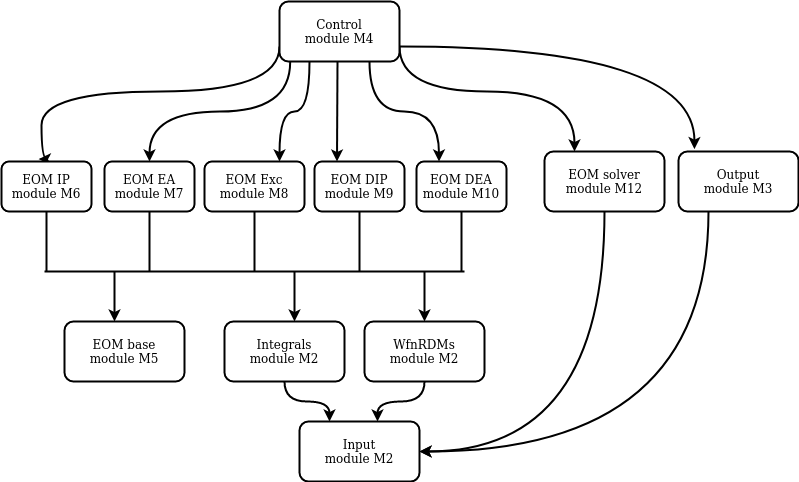
\includegraphics[width=0.7\textwidth]{UsesHierarchy.png}
\caption{Use hierarchy among modules}
\label{FigUH}
\end{figure}

%\section*{References}

\bibliographystyle {plainnat}
\bibliography{../../../refs/References}

\end{document}